Discretization information for DISL grids is read from the file that is specified by ``DISL6'' as the file type. The approach for numbering cell and cell vertices for the DISL Package is shown in figure~\ref{fig:disl_example}.  The list of vertices for a cell must be listed in the order that defines the line representing the cell. 

\begin{figure}[ht]
	\centering
	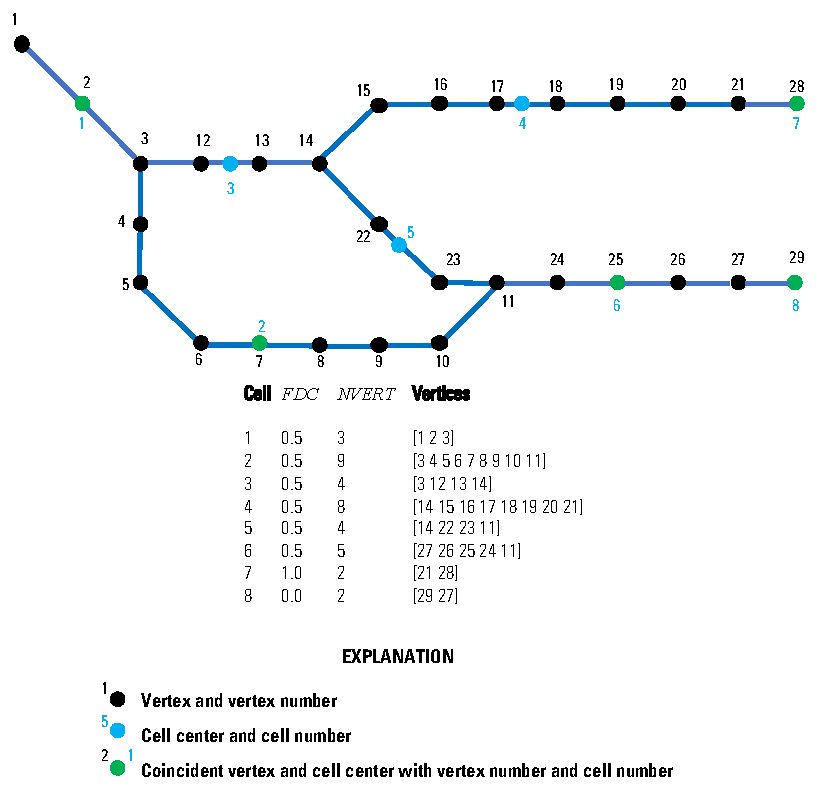
\includegraphics[scale=1.0]{Figures/DISL_example}
	\caption{Schematic diagram showing the vertices and cells defined using the Linear Discretization Package. The list of vertices used to define each cell ordered in either an upstream or downstream direction.  From \cite{modflow6gwf}}
	\label{fig:disl_example}
\end{figure}


\vspace{5mm}
\subsubsection{Structure of Blocks}
\lstinputlisting[style=blockdefinition]{./mf6ivar/tex/lnf-disl-options.dat}
\lstinputlisting[style=blockdefinition]{./mf6ivar/tex/lnf-disl-dimensions.dat}
\lstinputlisting[style=blockdefinition]{./mf6ivar/tex/lnf-disl-griddata.dat}
\lstinputlisting[style=blockdefinition]{./mf6ivar/tex/lnf-disl-vertices.dat}
\lstinputlisting[style=blockdefinition]{./mf6ivar/tex/lnf-disl-cell1d.dat}

\vspace{5mm}
\subsubsection{Explanation of Variables}
\begin{description}
% DO NOT MODIFY THIS FILE DIRECTLY.  IT IS CREATED BY mf6ivar.py 

\item \textbf{Block: OPTIONS}

\begin{description}
\item \texttt{length\_units}---is the length units used for this model.  Values can be ``FEET'', ``METERS'', or ``CENTIMETERS''.  If not specified, the default is ``UNKNOWN''.

\item \texttt{NOGRB}---keyword to deactivate writing of the binary grid file.

\item \texttt{xorigin}---x-position of the origin used for model grid vertices.  This value should be provided in a real-world coordinate system.  A default value of zero is assigned if not specified.  The value for XORIGIN does not affect the model simulation, but it is written to the binary grid file so that postprocessors can locate the grid in space.

\item \texttt{yorigin}---y-position of the origin used for model grid vertices.  This value should be provided in a real-world coordinate system.  If not specified, then a default value equal to zero is used.  The value for YORIGIN does not affect the model simulation, but it is written to the binary grid file so that postprocessors can locate the grid in space.

\item \texttt{angrot}---counter-clockwise rotation angle (in degrees) of the model grid coordinate system relative to a real-world coordinate system.  If not specified, then a default value of 0.0 is assigned.  The value for ANGROT does not affect the model simulation, but it is written to the binary grid file so that postprocessors can locate the grid in space.

\end{description}
\item \textbf{Block: DIMENSIONS}

\begin{description}
\item \texttt{nodes}---is the number of linear cells.

\item \texttt{nvert}---is the total number of (x, y, z) vertex pairs used to characterize the model grid.

\end{description}
\item \textbf{Block: GRIDDATA}

\begin{description}
\item \texttt{idomain}---is an optional array that characterizes the existence status of a cell.  If the IDOMAIN array is not specified, then all model cells exist within the solution.  If the IDOMAIN value for a cell is 0, the cell does not exist in the simulation.  Input and output values will be read and written for the cell, but internal to the program, the cell is excluded from the solution.  If the IDOMAIN value for a cell is 1, the cell exists in the simulation.

\end{description}
\item \textbf{Block: VERTICES}

\begin{description}
\item \texttt{iv}---is the vertex number.  Records in the VERTICES block must be listed in consecutive order from 1 to NVERT.

\item \texttt{xv}---is the x-coordinate for the vertex.

\item \texttt{yv}---is the y-coordinate for the vertex.

\item \texttt{zv}---is the z-coordinate for the vertex.

\end{description}
\item \textbf{Block: CELL1D}

\begin{description}
\item \texttt{icell1d}---is the cell1d number.  Records in the cell1d block must be listed in consecutive order from the first to the last.

\item \texttt{fdc}---is the fractional distance to the cell center. FDC is relative to the first vertex in the ICVERT array. In most cases FDC should be 0.5, which would place the center of the line segment that defines the cell. If the value of FDC is 1, the cell center would located at the last vertex. FDC values of 0 and 1 can be used to place the node at either end of the cell which can be useful for cells with boundary conditions.

\item \texttt{ncvert}---is the number of vertices required to define the cell.  There may be a different number of vertices for each cell.

\item \texttt{icvert}---is an array of integer values containing vertex numbers (in the VERTICES block) used to define the cell.  Vertices must be listed in the order that defines the line representing the cell.  Cells that are connected must share vertices. The bottom elevation of the cell is calculated using the ZV of the first and last vertex point and FDC.

\end{description}


\end{description}

\vspace{5mm}
\subsubsection{Example Input File}
\lstinputlisting[style=inputfile]{./mf6ivar/examples/lnf-disl-example.dat}
